\section{Đánh giá mô hình dự đoán}

\subsection{Các Phương pháp Đánh giá Hiệu quả Mô hình}

Để đánh giá hiệu quả của các mô hình học máy, bốn chỉ số phổ biến được sử dụng như sau:

\begin{itemize}
    \item \textbf{RMSE (Root Mean Square Error)}:
    \[
    RMSE = \sqrt{\frac{1}{n} \sum_{i=1}^{n} (y_i - \hat{y}_i)^2}
    \]

    \item \textbf{RRMSE (Relative RMSE)}:
    \[
    RRMSE = \frac{RMSE}{\overline{y}}
    \]

    \item \textbf{R-squared ($R^2$)}:
    \[
    R^2 = 1 - \frac{\sum_{i=1}^{n}(y_i - \hat{y}_i)^2}{\sum_{i=1}^{n}(y_i - \overline{y})^2}
    \]

    \item \textbf{MAE (Mean Absolute Error)}:
    \[
    MAE = \frac{1}{n} \sum_{i=1}^{n} |y_i - \hat{y}_i|
    \]
\end{itemize}

\subsection{Kết quả đánh giá}

Sau khi huấn luyện, nhóm thu được các chỉ số đánh giá như sau:

\begin{table}[H]
\centering
\caption{Các chỉ số đánh giá hiệu suất mô hình}
\begin{tabular}{|c|c|c|c|c|}
\hline
\textbf{Phương Pháp} & \textbf{RMSE} & \textbf{RRMSE} & \(\mathbf{R}^2\) & \textbf{MAE} \\
\hline
Linear Regression & 1,324,506.96 & 0.2645 & 0.653 & 970,043.40 \\
\hline
Random Forest & 1,400,619.50 & 0.2797 & 0.612 & 1,010,525.30 \\
\hline
XG\_Boost & 1,352,015.72 & 0.27 & 0.64 & 976,624.56 \\
\hline
Mạng Nơ-ron & 1,347,227.33 &0.27 & 0.64 & 956,810.86 \\
\hline
\end{tabular}
\end{table}

Dựa trên kết quả thu được, có thể rút ra các nhận xét chi tiết sau:

\begin{itemize}
	\item Mô hình \textbf{Hồi quy tuyến tính (Linear Regression)} đạt hiệu suất tổng thể tốt nhất dựa trên chỉ số RMSE thấp nhất ($1,324,506.96$) và hệ số xác định $R^2$ cao nhất ($0.653$). Điều này cho thấy tập dữ liệu có xu hướng phân bố tuyến tính khá mạnh, giúp một phương pháp cơ bản phát huy tối đa sức mạnh mà không gặp tình trạng quá khớp (overfitting).
	
	\item \textbf{Mạng Nơ-ron (MLP)} và \textbf{XGBoost} bám sát ngay sau với mức hiệu năng vô cùng ổn định ($R^2$ đều đạt mức $0.64$). Đáng chú ý, Mạng Nơ-ron lại là mô hình sở hữu sai số tuyệt đối trung bình (MAE) thấp nhất ($956,810.86$). Điều này chứng tỏ MLP có khả năng dự đoán các mức giá nhà thông thường rất sát với thực tế, dù thỉnh thoảng nhạy cảm với các điểm dị biệt (outliers) khiến chỉ số RMSE bị đẩy lên cao hơn so với Hồi quy tuyến tính.
	
	\item Mô hình \textbf{Random Forest} thể hiện hiệu suất kém nhất trong cả bốn phương pháp. Mặc dù là một thuật toán mạnh về khả năng mô hình hóa quan hệ phi tuyến, nhưng đối với tập dữ liệu này, thuật toán cây phân quyết định không mang lại hiệu quả, dẫn đến các chỉ số sai số cao nhất.
\end{itemize}

\textbf{Kết luận:} Dữ liệu trong bài toán mang đậm tính chất tuyến tính, do đó mô hình Hồi quy tuyến tính lại trở thành lựa chọn an toàn và hiệu quả nhất về mặt tổng thể. Tuy nhiên, nếu ưu tiên độ chính xác trên trung bình (dựa theo MAE), Mạng Nơ-ron nhiều lớp hoàn toàn là một giải pháp dự đoán đáng tin cậy.

\subsection{Đồ thị đánh giá}

Để trực quan hóa hiệu quả mô hình, nhóm sử dụng ba loại biểu đồ:

\begin{itemize}
    \item \textbf{Predictions vs Actual}: đánh giá độ chính xác tổng thể
    \item \textbf{Residuals vs Predicted}: kiểm tra lỗi hệ thống
    \item \textbf{Distribution of Residuals}: đánh giá phân phối sai số
\end{itemize}

\begin{figure}[H]
    \centering
    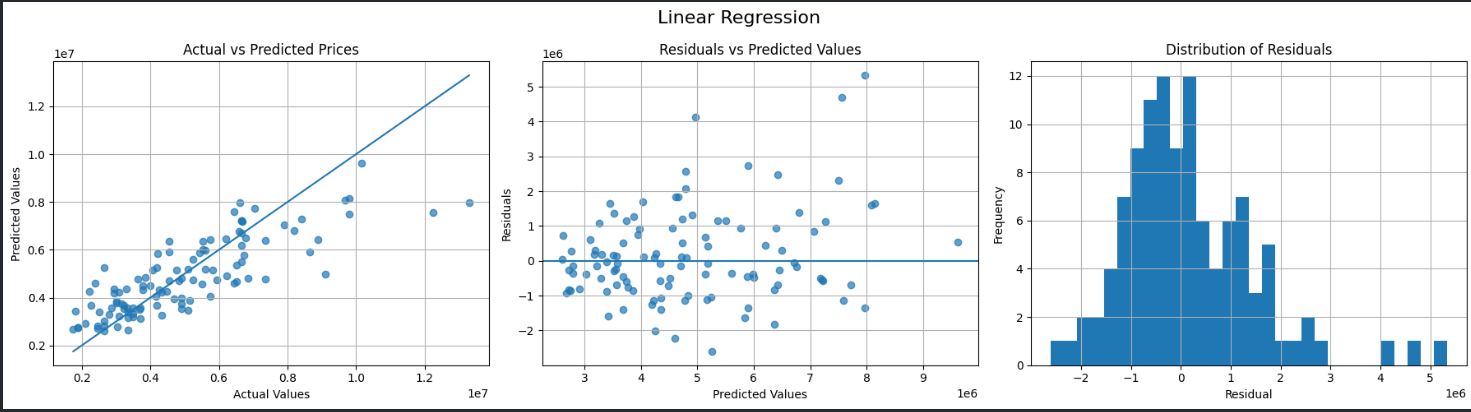
\includegraphics[width=0.95\textwidth]{chapters/Implement/linear_regression.png}
    \caption{Linear Regression: (a) Predictions vs Actual, (b) Residuals vs Predictions, (c) Distribution of Residuals}
    \label{fig:linear_eval}
\end{figure}

\begin{figure}[H]
    \centering
    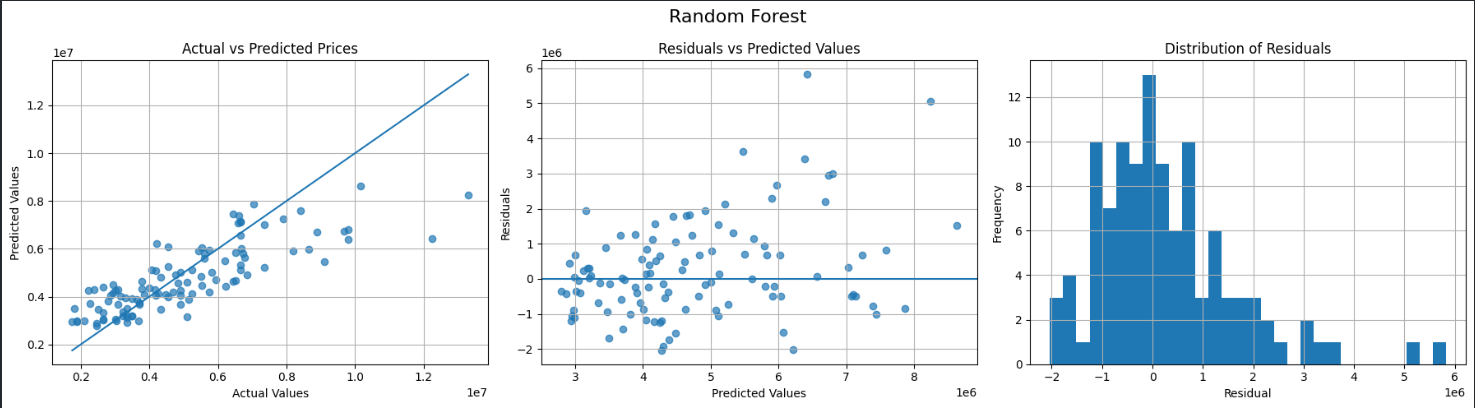
\includegraphics[width=0.95\textwidth]{chapters/Implement/random_forest.png}
    \caption{Random Forest: (a) Predictions vs Actual, (b) Residuals vs Predictions, (c) Distribution of Residuals}
    \label{fig:rf_eval}
\end{figure}

\begin{figure}[H]
	\centering
	\caption{XGBoost}
	
	\begin{minipage}{0.32\textwidth}
		\centering
		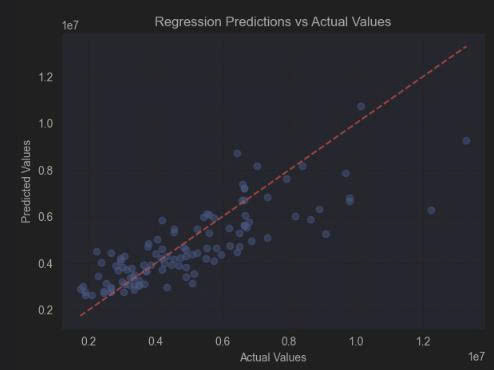
\includegraphics[width=\linewidth, height=6cm]{chapters/Preprocessing/images/xgb1.jpg}
		\textbf{(a) Predictions vs Actual}
		\label{fig:xgb_pred_vs_actual}
	\end{minipage}
	\hfill
	\begin{minipage}{0.32\textwidth}
		\centering
		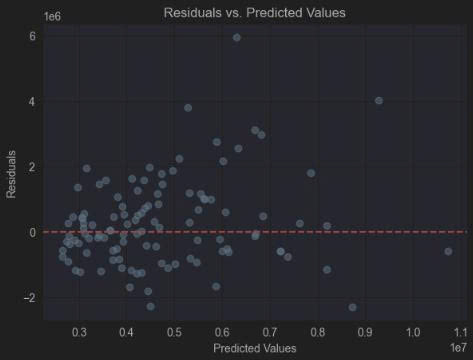
\includegraphics[width=\linewidth, height=6cm]{chapters/Preprocessing/images/xgb2.jpg}
		\textbf{(b) Residuals vs Predictions}
		\label{fig:xgb_residuals_vs_pred}
	\end{minipage}
	\hfill
	\begin{minipage}{0.32\textwidth}
		\centering
		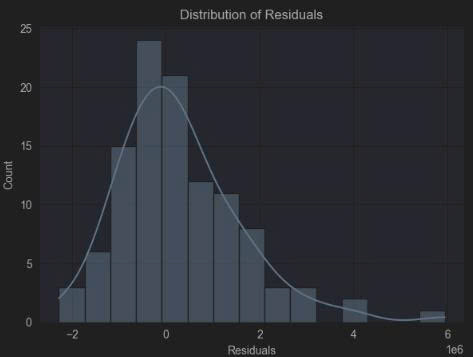
\includegraphics[width=\linewidth, height=6cm]{chapters/Preprocessing/images/xgb3.jpg}
		\textbf{(c) Distribution of Residuals}
		\label{fig:xgb_residuals_dist}
	\end{minipage}
\end{figure}


\begin{figure}[H]
	\centering
	\caption{Mạng Nơ-ron nhiều lớp}
	
	\begin{minipage}{0.32\textwidth}
		\centering
		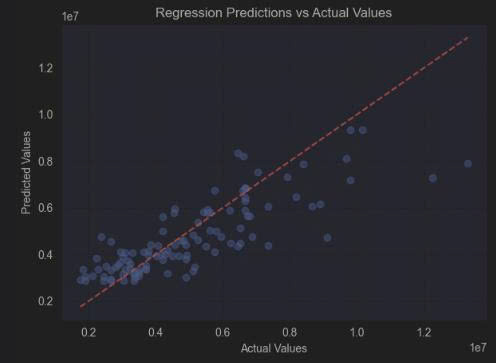
\includegraphics[width=\linewidth, height=6cm]{chapters/Preprocessing/images/mlp1.jpg}
		
		\textbf{(a) Regression Predictions vs Actual Values}
		\label{fig:regression}
	\end{minipage}
	\hfill
	\begin{minipage}{0.32\textwidth}
		\centering
		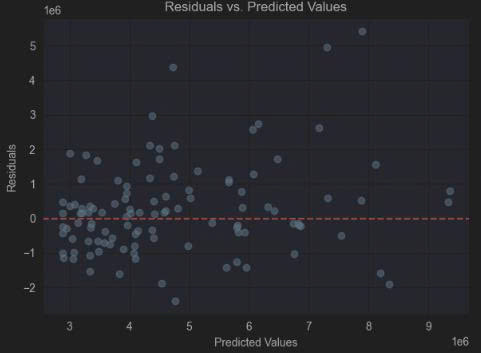
\includegraphics[width=\linewidth, height=6cm]{chapters/Preprocessing/images/mlp2.jpg}
		
		\textbf{(b) Residuals vs. Predicted Values}
		\label{fig:residuals_vs_pred}
	\end{minipage}
	\hfill
	\begin{minipage}{0.32\textwidth}
		\centering
		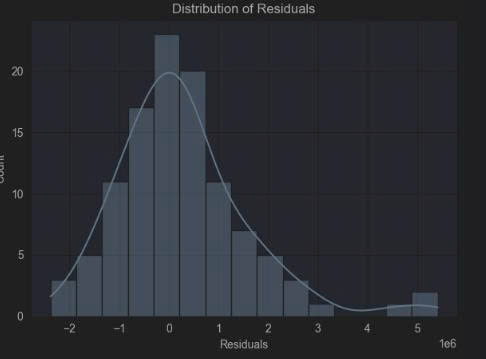
\includegraphics[width=\linewidth, height=6cm]{chapters/Preprocessing/images/mlp3.jpg}
		
		\textbf{(c) Distribution of Residuals}
		\label{fig:residual_distribution}
	\end{minipage}
\end{figure}

Từ các biểu đồ phân tích và giá trị dự đoán, có thể nhận thấy:

\begin{itemize}
	\item Với \textbf{Linear Regression}, các điểm dữ liệu phân bố khá sát đường lý tưởng $y = \hat{y}$. Phần dư phân bố ngẫu nhiên đều quanh trục 0 và biểu đồ phân phối phần dư có dạng hình quả chuông gần với phân phối chuẩn nhất, cho thấy mô hình dự đoán rất đồng đều và ổn định.
	
	\item Với \textbf{Random Forest}, độ phân tán của các điểm lớn hơn rõ rệt, đặc biệt phần dư có xu hướng loe rộng ra ở phân khúc các căn nhà có giá trị cao. Phân phối phần dư có xu hướng dẹt hơn, minh chứng cho việc mô hình gặp khó khăn và sai số lớn hơn so với mô hình tuyến tính.
	
	\item Với \textbf{XGBoost}, biểu đồ cho thấy sự cải thiện đáng kể so với Random Forest khi các điểm dự đoán bám sát đường lý tưởng hơn. Tuy nhiên, ở vùng giá trị cực đại, phần dư vẫn xuất hiện sự phân tán nhất định, chưa duy trì được độ hội tụ xuyên suốt như Linear Regression.
	
	\item Với \textbf{Mạng Nơ-ron (MLP)}, mật độ các điểm dữ liệu tập trung cực kỳ dày đặc và bám rất sát đường lý tưởng ở các phân khúc giá trung bình và thấp (phản ánh đúng việc mô hình đạt chỉ số MAE thấp nhất). Tuy nhiên, đồ thị phần dư cũng bộc lộ rõ một vài điểm dị biệt nằm rải rác khá xa trục 0, giải thích nguyên nhân chỉ số RMSE bị phạt nặng và cao hơn so với Hồi quy tuyến tính.
\end{itemize}

\subsection{Kết luận}

Thông qua quá trình huấn luyện, tối ưu hóa siêu tham số và đánh giá trực quan, nhóm có thể kết luận rằng \textbf{Hồi quy tuyến tính (Linear Regression)} là lựa chọn phù hợp và tối ưu nhất cho bài toán dự đoán giá nhà trên tập dữ liệu này. Nguyên nhân cốt lõi là do dữ liệu đầu vào thể hiện xu hướng tuyến tính rõ rệt, giúp một phương pháp thống kê cơ bản phát huy tối đa hiệu năng (RMSE thấp nhất, $R^2$ cao nhất), đồng thời tiết kiệm tuyệt đối chi phí tính toán.

Bên cạnh đó, \textbf{Mạng Nơ-ron nhiều lớp (MLP)} nổi lên như một giải pháp cực kỳ tiềm năng nếu hệ thống triển khai thực tế ưu tiên sai số tuyệt đối thấp nhất cho các căn nhà phổ thông (chỉ số MAE tốt nhất).

Ngược lại, các mô hình học máy theo dạng tập hợp phức tạp như Random Forest hay XGBoost lại không mang lại sự đột phá đáng kể về mặt độ chính xác, thậm chí tiêu tốn nhiều tài nguyên hơn cho việc tìm kiếm siêu tham số, do đó không phải là hướng tiếp cận hiệu quả nhất trong bối cảnh dữ liệu hiện tại.

\section{Tổng Kết}
Trong bài tập lớn lần này, nhóm đã tiến hành đầy đủ các bước trong quy trình khai phá tri thức nhằm tìm ra mô hình phù hợp nhất để giải quyết bài toán dự đoán giá nhà, sử dụng tập dữ liệu gồm 545 ngôi nhà với các thuộc tính đặc trưng có giá trị cho quá trình huấn luyện.

Từ dữ liệu thô thu thập được trên nền tảng Kaggle, nhóm đã lần lượt thực hiện các bước: làm sạch dữ liệu, tích hợp dữ liệu, chọn lọc thuộc tính, chuyển đổi dữ liệu, khai phá dữ liệu, đánh giá mô hình và biểu diễn tri thức. Bốn phương pháp khai phá dữ liệu được áp dụng gồm: Hồi quy tuyến tính, Random Forest, XGBoost và mạng Nơ-ron nhiều lớp (Neural Network), nhằm so sánh và lựa chọn mô hình tối ưu.

Thông qua quá trình huấn luyện và đánh giá, cả bốn mô hình đều cho kết quả khả quan. Tuy nhiên, mô hình \textbf{Hồi quy tuyến tính (Linear Regression)} thể hiện hiệu năng tổng thể vượt trội nhất (đạt chỉ số RMSE thấp nhất và $R^2$ cao nhất). Điều này xuất phát từ việc các đặc trưng trong tập dữ liệu mang đậm tính chất tuyến tính, giúp một mô hình thống kê cơ bản phát huy tối đa sức mạnh, đảm bảo khả năng tổng quát hóa cao mà không bị rơi vào trạng thái quá khớp (overfitting). 

Bên cạnh đó, \textbf{Mạng Nơ-ron nhiều lớp (MLP)} cũng là một điểm sáng đáng ghi nhận khi đạt mức sai số tuyệt đối trung bình (MAE) thấp nhất trong cả bốn phương pháp, cho thấy khả năng dự đoán cực kỳ sát sao đối với các phân khúc nhà phổ thông. Mô hình \textbf{XGBoost} xếp ngay sau với sự hội tụ ổn định và độ tin cậy cao.

Tóm lại, để triển khai trong hệ thống dự đoán giá nhà thực tế, Hồi quy tuyến tính là lựa chọn ưu tiên hàng đầu nhờ sự cân bằng hoàn hảo giữa độ chính xác, chi phí tài nguyên tính toán thấp và tính dễ diễn giải. Nếu hệ thống đặc thù yêu cầu tối thiểu hóa sai số tuyệt đối trên từng căn nhà cụ thể, mạng Nơ-ron sẽ là một phương án triển khai xuất sắc.